\documentclass[11pt]{article}

\usepackage[utf8]{inputenc}\usepackage[T1]{fontenc}
\usepackage{amsmath,amsthm,amssymb,enumitem,booktabs,xcolor,tikz,longtable,array,needspace,graphicx}
\usepackage{geometry}
\newcommand{\sect}[1]{\par\medskip\noindent\textbf{\large #1}\par\smallskip}
\theoremstyle{definition}\newtheorem*{example}{Example}\newtheorem*{method*}{Method}
\theoremstyle{remark}\newtheorem*{remark}{Remark}

\geometry{letterpaper,margin=1in}
\setlength{\parindent}{0pt}\setlength{\parskip}{0.5em}
\newcommand{\mk}[1]{}
\begin{document}
{\Large\textbf{The table as a map of configurations}}\\ Honors Chemistry $\cdot$ Unit 3 $\cdot$ Slot 14 $\cdot$ typed notes\par\medskip
\noindent\fbox{\parbox{\dimexpr\linewidth-2\fboxsep-2\fboxrule}{\textbf{Big question.} If I tell you only where an element sits on the table, what can you say about its electrons?}}\par\medskip

\sect{The table was a map before anyone could read it}
In 1869 Mendeleev set the elements in rows by mass and by how they behaved, and left gaps for elements nobody had found. It worked, and nobody knew why. Around 1913 Moseley showed that the true order was by atomic number. Within about fifteen years the shell model gave the reason: the rows are shells filling and the columns are the electrons left over in the outer shell. Today we draw the table from the configurations we wrote in slots 9 and 10, and then read it backwards.

\sect{A. Build the table from the ladder}
Fill the subshells in the order from slot 9: $1s,\ 2s,\ 2p,\ 3s,\ 3p,\ 4s,\ 3d,\ 4p$. Start a new row each time the outer shell number goes up. That gives four rows.\par\medskip
\begin{center}\begin{tabular}{@{}clc@{}}\toprule Period (outer shell) & Subshells that fill, in order & Elements\\\midrule
1 & $1s$ & 2\\
2 & $2s\;2p$ & 8\\
3 & $3s\;3p$ & 8\\
4 & $4s\;3d\;4p$ & 18\\\bottomrule\end{tabular}\end{center}
\begin{description}[leftmargin=1.2em,itemsep=2pt]
\item[Period] A row. Its number is the outer shell number, so period 3 means the outer electrons are in shell 3.
\item[Block] The subshell that fills last. The $s$ block is groups 1 and 2. The $p$ block is groups 13 to 18. The $d$ block is groups 3 to 12.
\end{description}\par
\textbf{The $d$ subshell is one shell behind its period.} The $3d$ boxes fill after $4s$, so they sit in period 4.
\begin{remark}[Going deeper]The $f$ block works the same way: $4f$ fills after $6s$, so those 14 columns sit under the table. We only name it today.\end{remark}

\begin{center}\resizebox{\linewidth}{!}{%
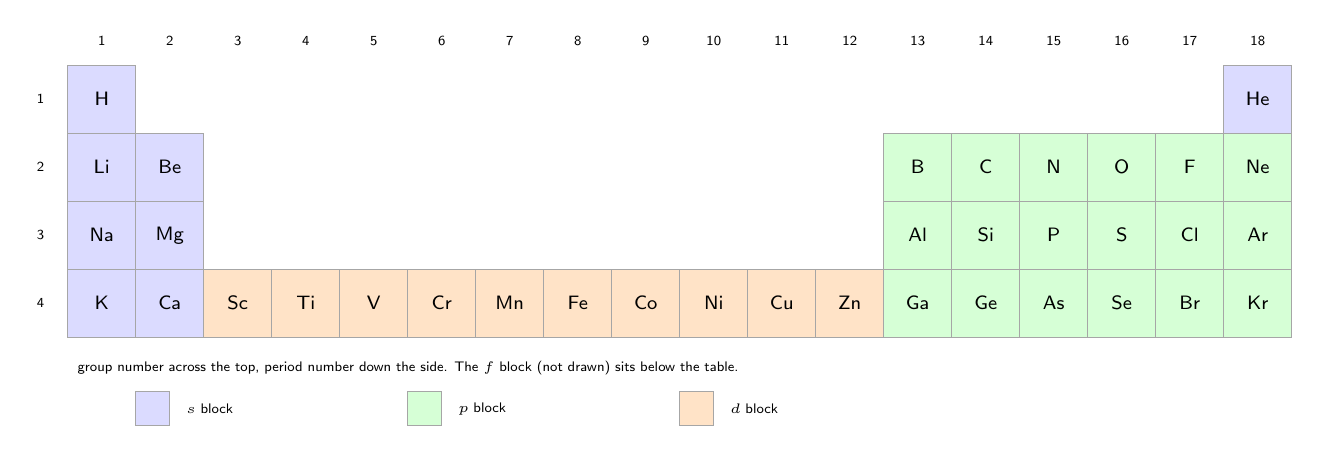
\begin{tikzpicture}[x=0.34in,y=-0.34in,every node/.style={font=\scriptsize\sffamily}]
\node[font=\tiny\sffamily] at (0.50,-0.35) {1};
\node[font=\tiny\sffamily] at (1.50,-0.35) {2};
\node[font=\tiny\sffamily] at (2.50,-0.35) {3};
\node[font=\tiny\sffamily] at (3.50,-0.35) {4};
\node[font=\tiny\sffamily] at (4.50,-0.35) {5};
\node[font=\tiny\sffamily] at (5.50,-0.35) {6};
\node[font=\tiny\sffamily] at (6.50,-0.35) {7};
\node[font=\tiny\sffamily] at (7.50,-0.35) {8};
\node[font=\tiny\sffamily] at (8.50,-0.35) {9};
\node[font=\tiny\sffamily] at (9.50,-0.35) {10};
\node[font=\tiny\sffamily] at (10.50,-0.35) {11};
\node[font=\tiny\sffamily] at (11.50,-0.35) {12};
\node[font=\tiny\sffamily] at (12.50,-0.35) {13};
\node[font=\tiny\sffamily] at (13.50,-0.35) {14};
\node[font=\tiny\sffamily] at (14.50,-0.35) {15};
\node[font=\tiny\sffamily] at (15.50,-0.35) {16};
\node[font=\tiny\sffamily] at (16.50,-0.35) {17};
\node[font=\tiny\sffamily] at (17.50,-0.35) {18};
\node[font=\tiny\sffamily] at (-0.4,0.50) {1};
\node[font=\tiny\sffamily] at (-0.4,1.50) {2};
\node[font=\tiny\sffamily] at (-0.4,2.50) {3};
\node[font=\tiny\sffamily] at (-0.4,3.50) {4};
\fill[blue!14] (0,0) rectangle (1,1);\draw[gray!70,line width=0.3pt] (0,0) rectangle (1,1);
\node at (0.50,0.50) {H};
\fill[blue!14] (17,0) rectangle (18,1);\draw[gray!70,line width=0.3pt] (17,0) rectangle (18,1);
\node at (17.50,0.50) {He};
\fill[blue!14] (0,1) rectangle (1,2);\draw[gray!70,line width=0.3pt] (0,1) rectangle (1,2);
\node at (0.50,1.50) {Li};
\fill[blue!14] (1,1) rectangle (2,2);\draw[gray!70,line width=0.3pt] (1,1) rectangle (2,2);
\node at (1.50,1.50) {Be};
\fill[green!16] (12,1) rectangle (13,2);\draw[gray!70,line width=0.3pt] (12,1) rectangle (13,2);
\node at (12.50,1.50) {B};
\fill[green!16] (13,1) rectangle (14,2);\draw[gray!70,line width=0.3pt] (13,1) rectangle (14,2);
\node at (13.50,1.50) {C};
\fill[green!16] (14,1) rectangle (15,2);\draw[gray!70,line width=0.3pt] (14,1) rectangle (15,2);
\node at (14.50,1.50) {N};
\fill[green!16] (15,1) rectangle (16,2);\draw[gray!70,line width=0.3pt] (15,1) rectangle (16,2);
\node at (15.50,1.50) {O};
\fill[green!16] (16,1) rectangle (17,2);\draw[gray!70,line width=0.3pt] (16,1) rectangle (17,2);
\node at (16.50,1.50) {F};
\fill[green!16] (17,1) rectangle (18,2);\draw[gray!70,line width=0.3pt] (17,1) rectangle (18,2);
\node at (17.50,1.50) {Ne};
\fill[blue!14] (0,2) rectangle (1,3);\draw[gray!70,line width=0.3pt] (0,2) rectangle (1,3);
\node at (0.50,2.50) {Na};
\fill[blue!14] (1,2) rectangle (2,3);\draw[gray!70,line width=0.3pt] (1,2) rectangle (2,3);
\node at (1.50,2.50) {Mg};
\fill[green!16] (12,2) rectangle (13,3);\draw[gray!70,line width=0.3pt] (12,2) rectangle (13,3);
\node at (12.50,2.50) {Al};
\fill[green!16] (13,2) rectangle (14,3);\draw[gray!70,line width=0.3pt] (13,2) rectangle (14,3);
\node at (13.50,2.50) {Si};
\fill[green!16] (14,2) rectangle (15,3);\draw[gray!70,line width=0.3pt] (14,2) rectangle (15,3);
\node at (14.50,2.50) {P};
\fill[green!16] (15,2) rectangle (16,3);\draw[gray!70,line width=0.3pt] (15,2) rectangle (16,3);
\node at (15.50,2.50) {S};
\fill[green!16] (16,2) rectangle (17,3);\draw[gray!70,line width=0.3pt] (16,2) rectangle (17,3);
\node at (16.50,2.50) {Cl};
\fill[green!16] (17,2) rectangle (18,3);\draw[gray!70,line width=0.3pt] (17,2) rectangle (18,3);
\node at (17.50,2.50) {Ar};
\fill[blue!14] (0,3) rectangle (1,4);\draw[gray!70,line width=0.3pt] (0,3) rectangle (1,4);
\node at (0.50,3.50) {K};
\fill[blue!14] (1,3) rectangle (2,4);\draw[gray!70,line width=0.3pt] (1,3) rectangle (2,4);
\node at (1.50,3.50) {Ca};
\fill[orange!22] (2,3) rectangle (3,4);\draw[gray!70,line width=0.3pt] (2,3) rectangle (3,4);
\node at (2.50,3.50) {Sc};
\fill[orange!22] (3,3) rectangle (4,4);\draw[gray!70,line width=0.3pt] (3,3) rectangle (4,4);
\node at (3.50,3.50) {Ti};
\fill[orange!22] (4,3) rectangle (5,4);\draw[gray!70,line width=0.3pt] (4,3) rectangle (5,4);
\node at (4.50,3.50) {V};
\fill[orange!22] (5,3) rectangle (6,4);\draw[gray!70,line width=0.3pt] (5,3) rectangle (6,4);
\node at (5.50,3.50) {Cr};
\fill[orange!22] (6,3) rectangle (7,4);\draw[gray!70,line width=0.3pt] (6,3) rectangle (7,4);
\node at (6.50,3.50) {Mn};
\fill[orange!22] (7,3) rectangle (8,4);\draw[gray!70,line width=0.3pt] (7,3) rectangle (8,4);
\node at (7.50,3.50) {Fe};
\fill[orange!22] (8,3) rectangle (9,4);\draw[gray!70,line width=0.3pt] (8,3) rectangle (9,4);
\node at (8.50,3.50) {Co};
\fill[orange!22] (9,3) rectangle (10,4);\draw[gray!70,line width=0.3pt] (9,3) rectangle (10,4);
\node at (9.50,3.50) {Ni};
\fill[orange!22] (10,3) rectangle (11,4);\draw[gray!70,line width=0.3pt] (10,3) rectangle (11,4);
\node at (10.50,3.50) {Cu};
\fill[orange!22] (11,3) rectangle (12,4);\draw[gray!70,line width=0.3pt] (11,3) rectangle (12,4);
\node at (11.50,3.50) {Zn};
\fill[green!16] (12,3) rectangle (13,4);\draw[gray!70,line width=0.3pt] (12,3) rectangle (13,4);
\node at (12.50,3.50) {Ga};
\fill[green!16] (13,3) rectangle (14,4);\draw[gray!70,line width=0.3pt] (13,3) rectangle (14,4);
\node at (13.50,3.50) {Ge};
\fill[green!16] (14,3) rectangle (15,4);\draw[gray!70,line width=0.3pt] (14,3) rectangle (15,4);
\node at (14.50,3.50) {As};
\fill[green!16] (15,3) rectangle (16,4);\draw[gray!70,line width=0.3pt] (15,3) rectangle (16,4);
\node at (15.50,3.50) {Se};
\fill[green!16] (16,3) rectangle (17,4);\draw[gray!70,line width=0.3pt] (16,3) rectangle (17,4);
\node at (16.50,3.50) {Br};
\fill[green!16] (17,3) rectangle (18,4);\draw[gray!70,line width=0.3pt] (17,3) rectangle (18,4);
\node at (17.50,3.50) {Kr};
\node[font=\tiny\sffamily,anchor=west] at (0,4.45) {group number across the top, period number down the side. The $f$ block (not drawn) sits below the table.};
\fill[blue!14] (1,4.8) rectangle (1.5,5.3);\draw[gray!70,line width=0.3pt] (1,4.8) rectangle (1.5,5.3);\node[anchor=west,font=\tiny\sffamily] at (1.6,5.05) {$s$ block};
\fill[green!16] (5,4.8) rectangle (5.5,5.3);\draw[gray!70,line width=0.3pt] (5,4.8) rectangle (5.5,5.3);\node[anchor=west,font=\tiny\sffamily] at (5.6,5.05) {$p$ block};
\fill[orange!22] (9,4.8) rectangle (9.5,5.3);\draw[gray!70,line width=0.3pt] (9,4.8) rectangle (9.5,5.3);\node[anchor=west,font=\tiny\sffamily] at (9.6,5.05) {$d$ block};
\end{tikzpicture}}
\end{center}


\sect{B. Valence configuration from position}
\begin{method*}
1.\ Find the period $n$ and the group $g$.\par
2.\ Name the block: groups 1 and 2 are $s$, groups 13 to 18 are $p$.\par
3.\ Group 1 gives $ns^{1}$. Group 2 gives $ns^{2}$. Groups 13 to 18 give $ns^{2}np^{\,g-12}$.\par
4.\ Valence electrons: $g$ for groups 1 and 2, and $g-10$ for groups 13 to 18.
\end{method*}
\textbf{One exception.} Helium is in group 18 but it is $1s^{2}$, with only 2 valence electrons, because there is no $1p$ subshell.
\begin{remark}[Common mistake]In period 4, the valence configuration of a $p$-block atom is $4s$ and $4p$ only. The $3d^{10}$ is full and is not counted. Slot 10 said valence means the outer shell.\end{remark}

\sect{Worked together}
\begin{example}[Sulfur, together]Sulfur is in period 3, group 16. Group 16 is in the $p$ block, so the valence configuration is $ns^{2}np^{\,g-12}=3s^{2}3p^{4}$. Valence electrons: $16-10=6$.\end{example}
\begin{example}[Gallium, first step done]Gallium is in period 4, group 13. It is in the $p$ block. Finish it: $4s^{2}4p^{1}$, with $13-10=3$ valence electrons.\end{example}

\sect{What to copy}
\begin{enumerate}[label=\textbf{Copy \arabic*.},leftmargin=4.2em,itemsep=2pt]
\item Period = row = the outer shell number. Rows hold 2, 8, 8, 18.
\item Block = the subshell filling last: $s$ is groups 1--2, $p$ is groups 13--18, $d$ is groups 3--12.
\item The $d$ subshell is one shell behind its period: $3d$ sits in period 4.
\item Group 1: $ns^{1}$. Group 2: $ns^{2}$.
\item Groups 13--18: $ns^{2}np^{\,g-12}$, where $g$ is the group number.
\item Valence electrons: groups 1--2 equal $g$; groups 13--18 equal $g-10$.
\item Helium is in group 18 but is $1s^{2}$: 2 valence electrons.
\item Sulfur: period 3, group 16 gives $3s^{2}3p^{4}$ (6 valence).
\item Gallium: period 4, group 13 gives $4s^{2}4p^{1}$ (3 valence).
\end{enumerate}
\bigskip\noindent\textbf{Back to the big question.} Position on the table gives the period (the outer shell), the block (the subshell filling last) and, in the main groups, the valence configuration. The table is the configuration pattern drawn on a page.
\sect{Up next}
Lithium and sodium both end in $s^{1}$, and both react the same way. But sodium gives up its outer electron more easily. Why is sodium's outer electron easier to remove than lithium's?
\end{document}